\documentclass[11pt]{article}
\usepackage[letterpaper,margin=1in]{geometry}
\usepackage[T1]{fontenc}
\usepackage{newtxtext,newtxmath}
\usepackage{microtype}
\usepackage{graphicx}
\usepackage{booktabs}
\usepackage{tabularx}
\usepackage{array}
\usepackage[font=small,labelfont=bf,skip=6pt]{caption}
\usepackage{subcaption}
\usepackage{float}
\usepackage{xcolor}
\usepackage{titlesec}
\usepackage{fancyhdr}
\usepackage[hidelinks]{hyperref}

\graphicspath{{../report-assets/}}
\definecolor{ink}{HTML}{201F1D}
\definecolor{gold}{HTML}{8A6020}
\hypersetup{colorlinks=true,linkcolor=ink,urlcolor=gold,citecolor=ink}

\titleformat{\section}{\large\bfseries}{\thesection}{0.8em}{}
\titleformat{\subsection}{\normalsize\bfseries}{\thesubsection}{0.8em}{}
\titlespacing*{\section}{0pt}{14pt}{6pt}
\titlespacing*{\subsection}{0pt}{10pt}{4pt}
\setlength{\parskip}{4pt}
\renewcommand{\arraystretch}{1.18}
\newcolumntype{L}{>{\raggedright\arraybackslash}X}
\newcolumntype{P}[1]{>{\raggedright\arraybackslash}p{#1}}
\renewcommand{\topfraction}{0.9}
\renewcommand{\bottomfraction}{0.8}
\renewcommand{\textfraction}{0.1}
\renewcommand{\floatpagefraction}{0.85}
\setcounter{topnumber}{3}
\setcounter{totalnumber}{4}

\pagestyle{fancy}
\fancyhf{}
\fancyhead[L]{\small LeadFinder: Technical Project Report}
\fancyhead[R]{\small ENMGT 4405}
\fancyfoot[C]{\small\thepage}
\renewcommand{\headrulewidth}{0.4pt}

\newcommand{\code}[1]{\texttt{\small #1}}

\begin{document}

\thispagestyle{plain}
\begin{center}
{\small ENMGT 4405 \quad Final Project \quad Technical Project Report}\\[10pt]
{\LARGE\bfseries LeadFinder}\\[6pt]
{\large An AI lead finder for health-tech sales to independent medical practices}\\[12pt]
Daniel Akinwale \quad Mahika Arora \quad Hanna Malet\\ Gabriel Maurad \quad Ashwin Prajeeth \quad Sasha Shkolnikov\\[4pt]
{\small November 2026 \quad\textbullet\quad Live demo: \href{https://leadfinder-mauve.vercel.app}{leadfinder-mauve.vercel.app}}\\{\small SDR logins \code{riley} and \code{jo}, sales manager \code{morgan}; the password is on the login page}\\[6pt]{\small\itshape Written by Claude (Anthropic) from the team's inputs and information; see the AI attribution on page~\pageref{sec:ai-attribution}.}
\end{center}
\vspace{4pt}

\begin{abstract}
\noindent LeadFinder ranks independent medical practices by their chance of buying a health-tech product, so that a sales development rep (SDR) contacts the right practice first, and it drafts outreach that a person approves before anything is sent. The system is a FastAPI service with SQLite storage that combines a deterministic visit-intent gate, a logistic regression over 21 practice and visit facts, Claude for the first email and call brief, code checks on every draft, and a logged human decision on every lead. A bounded Claude research agent over a table of 742 real practices from the public NPI registry, and a fixed LangGraph graph that orchestrates the whole pipeline, are built and tested but not yet called by the web app. On 2,400 held-out simulated leads the model's top tenth converts at 77.9\% against a 28.7\% base rate, a 2.72$\times$ lift, with a calibration error of 1.7 points; testing also reduced browser false passes at the gate from 15.7\% to 0\% and raised correct practice matches on real registry names from 63.1\% to 91.5\% with no wrong matches. Since every conversion label is simulated, these results compare scorers with one another and confirm that each module behaves as designed, rather than forecasting real sales.
\end{abstract}

\section{Problem statement and motivation}

A health-tech company selling to independent medical practices has tens of thousands of possible customers in the United States and an SDR team that can only contact a small share of them each month, so the order in which practices are contacted matters more than the length of the list. A good lead contacted a week late goes cold, and an hour spent researching a practice that was never a fit is an hour not spent selling. The question LeadFinder answers is therefore narrow: given who visited the seller's website and what is publicly known about each practice, which practice should an SDR call first, and what should they say?

Today a lead passes through three manual hand-offs before anyone talks to it. A website tracking tool identifies the visiting company but makes no judgment about fit; marketing then applies a hand-set points threshold, and qualified leads wait in a queue; finally an SDR researches each practice by hand before reaching out, often for hours on practices that were never a fit. Each hand-off adds delay, and the points threshold is a set of guesses that nobody checks against outcomes. In the case study we used for sizing, an SDR spends about 30 minutes per lead and a team of 12 works roughly 500 leads a month, converting 36 of them, or 7.2\%.

Existing tools do not close this gap at a price a small seller can pay. HubSpot costs about \$20 a seat a month and already ships a prospecting agent that drafts email, but its scoring only sees the customer's own portal data and models nothing about a practice's specialty, size or EHR. Definitive Healthcare offers rich physician and claims data, but contracts start at roughly \$25,000 to \$60,000 a year, and generic contact databases such as Apollo and Clay are reported to perform poorly in healthcare (prices as cited in our proposal, not measured by us). One concern this raised early in the project is that automating outreach was not a new idea on its own, which pushed the design toward the things these tools lack: healthcare-specific practice data, scores that explain themselves, and accuracy that is measured rather than claimed.

\section{From research to design}

Each finding from our brainstorm and proposal became a concrete design decision, and each decision can be seen on a specific page of the demo. The project moved from a brainstorm in early November that mapped how B2B leads move from tracker to marketing to SDR, through a proposal on November 8 that split the work into one role per manual hand-off, to architecture notes on November 14 and a build from November 15 to 18. The largest pivot came between the first two stages, when competitive research showed that HubSpot already drafts outreach with an AI agent; the project's edge then had to be the data and the honesty of the score rather than automation for its own sake.

The first finding was that generic tools ignore what defines a practice, so LeadFinder scores on specialty, size and EHR drawn from the public NPI registry. The second was that healthcare purchases involve several people and that reps will not act on a score they cannot check, so every score in the app lists the facts that moved it and where each fact came from. The third came from a vendor comparison reporting 8 to 15\% reply rates for human-plus-AI outreach against 1 to 3\% for fully autonomous agents, which is why an SDR approves, edits or rejects every email rather than the system sending on its own. The fourth was regulatory: email to practices is a CAN-SPAM question rather than a HIPAA one as long as no patient data enters, so only public business facts reach a model and every draft carries a postal address and an opt-out. The fifth was that buying intent shows in which pages a visitor reads, which became the tiered, rule-based visit-intent gate.

The finding that shaped the architecture most came from the course rather than the market. If each step of a pipeline works 90\% of the time, five chained steps work only $0.9^5 = 59\%$ of the time, so every place an LLM replaces a rule costs reliability that its judgment has to earn back. We therefore applied the course's test for when a step should be an agent (autonomy, a poorly defined task, and reasoning from context) to every step of the pipeline. Visit analysis fails that test, since its inputs are structured and its steps are known, so it is plain code; prospect research passes it, since name variants and ambiguous matches need judgment, so it is a bounded agent. The proposal also left one question open that we carried through the build, namely whether a transparent ML model ranks leads better than an LLM's own judgment, and Section~\ref{sec:results} reports the half of that comparison we have been able to run.

\section{Architecture}

LeadFinder runs one lead through nine steps in a fixed order, and only three of them use AI: the research agent, the scoring model and the writer. Figure~\ref{fig:workflow} shows that path, with each step colored by who performs it and marked by whether it is live in the demo, built beside the app, or planned.

\begin{figure}[htbp]
\centering
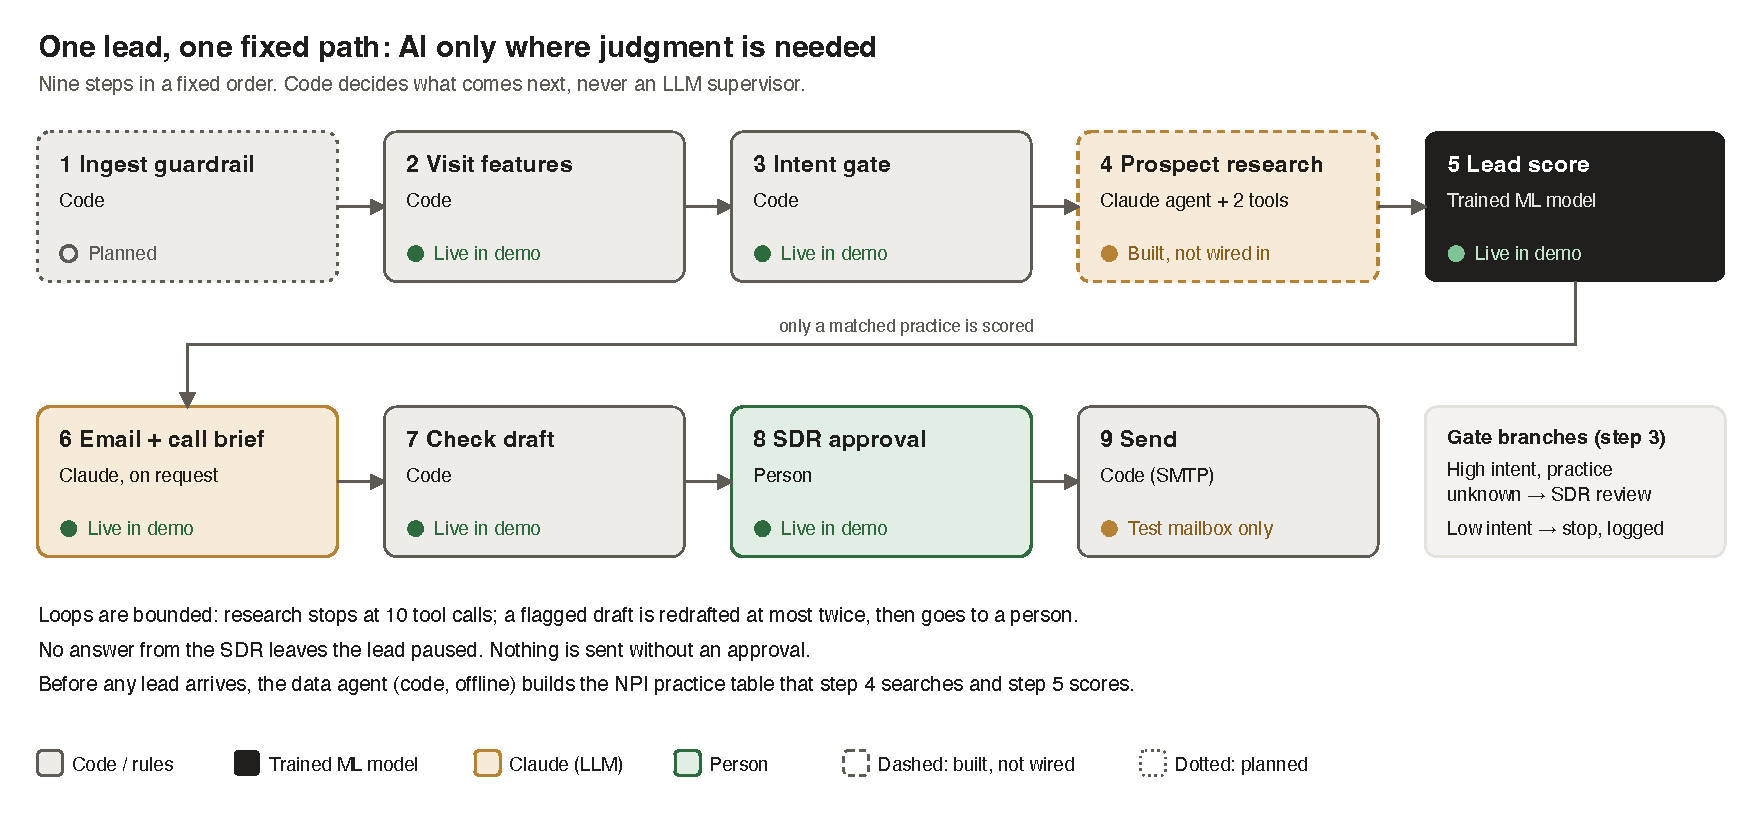
\includegraphics[width=\textwidth]{workflow.pdf}
\caption{The workflow for one lead. Grey steps are code, black is the trained model, gold is Claude and green is a person; dashed borders mark steps that are built and tested but not yet wired into the app, and the dotted border marks a planned step.}
\label{fig:workflow}
\end{figure}

Two choices in Figure~\ref{fig:workflow} carry most of the reliability argument. First, orchestration is a fixed graph rather than an LLM supervisor, since the order of steps never changes and a supervisor would add a point of failure without adding judgment. Second, the only loops are bounded: the research agent stops after 10 tool calls, and a draft that fails its checks is rewritten at most twice before it goes to a person, so a lead can neither cycle indefinitely nor be sent without an approval. The intent gate also has two exits besides research. A visitor with real intent whose practice cannot be identified goes to an SDR identity-review queue instead of being dropped, and low-intent traffic stops with a logged reason.

\begin{figure}[htbp]
\centering
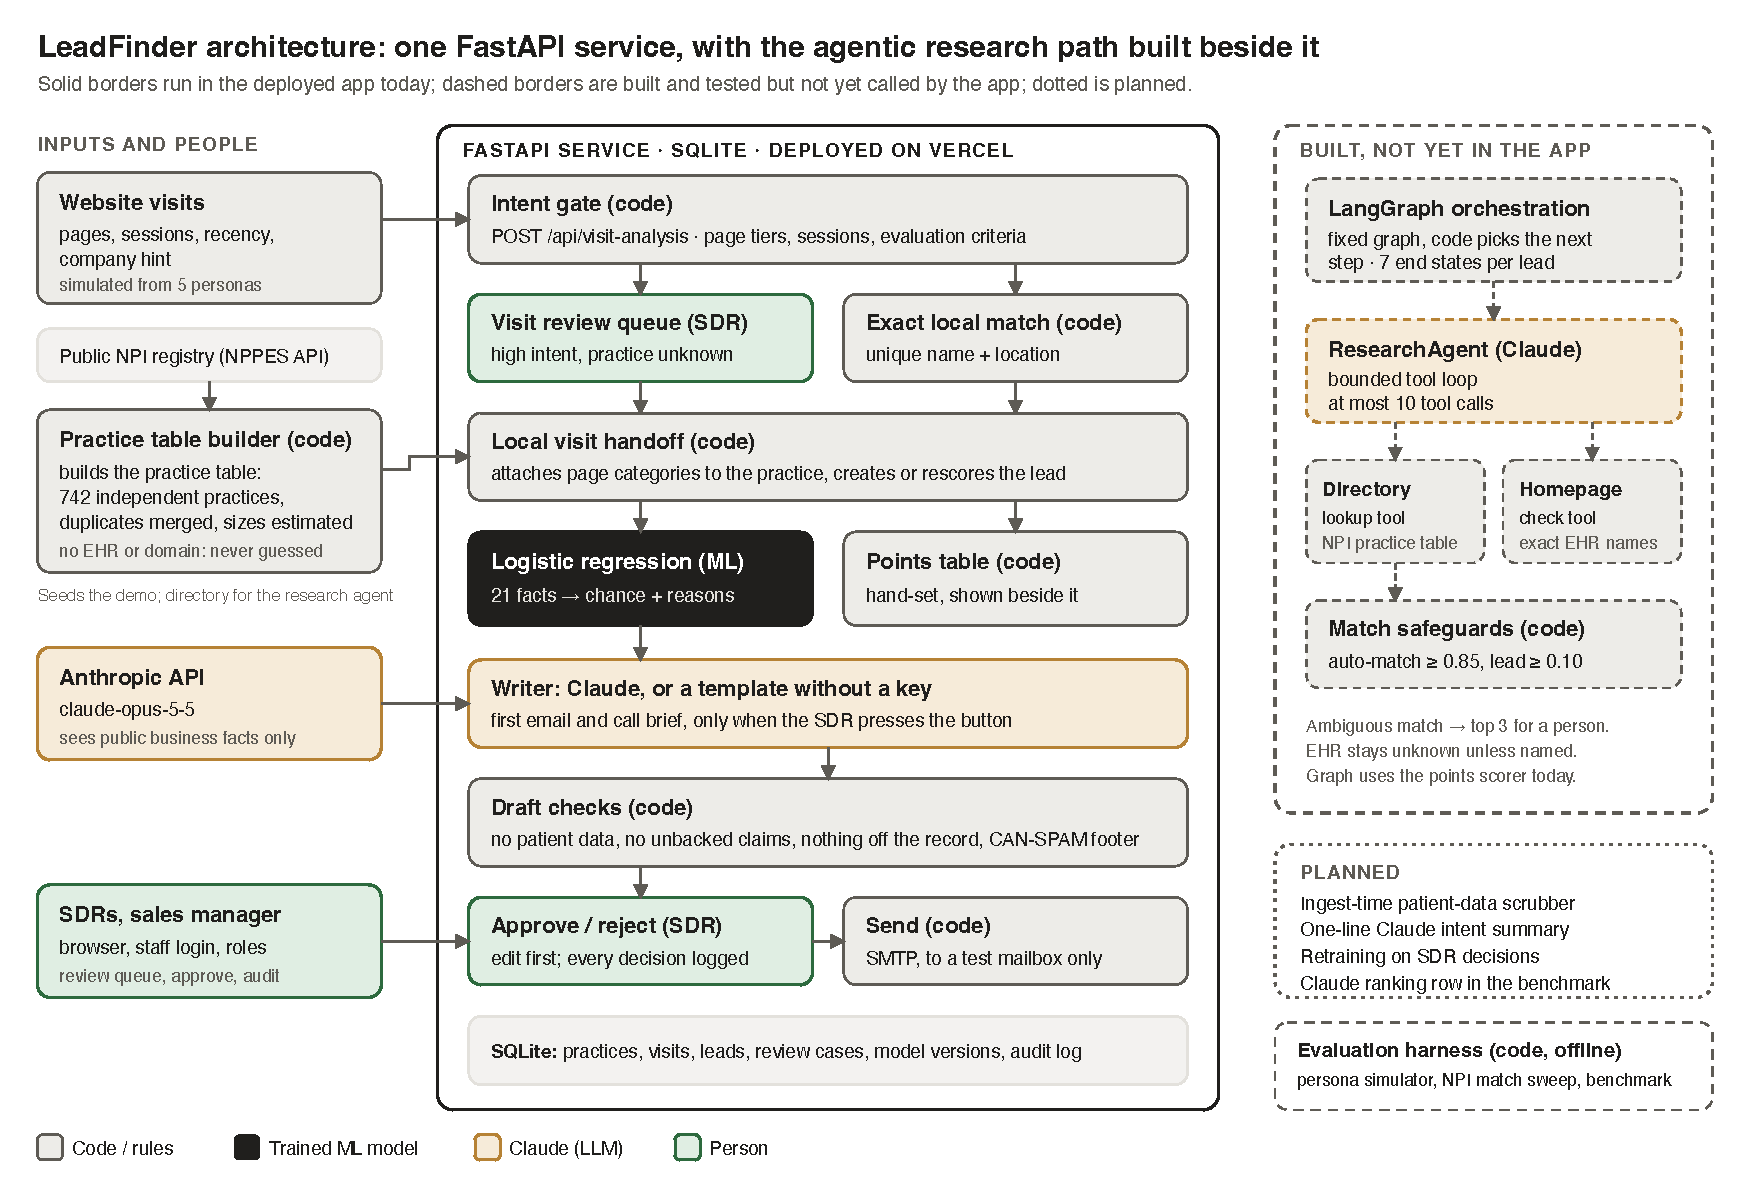
\includegraphics[width=0.94\textwidth]{architecture.pdf}
\caption{System architecture. The FastAPI service in the middle is what the deployed demo runs; the research agent and LangGraph graph on the right are merged with tests but are not yet called by the app.}
\label{fig:architecture}
\end{figure}

As Figure~\ref{fig:architecture} shows, the deployed system is a single FastAPI service with server-rendered pages and SQLite storage, hosted on Vercel, with password logins under two roles, SDR and sales manager. It takes three inputs: website visits, simulated from five buyer personas since we have no tracking feed; the practice record, drawn from 40 synthetic practices by default or from 742 real NPI practices with one setting; and, for the research agent only, a matched practice's own homepage. Anthropic's API is called only for writing on request and for the research agent's decisions, and in both cases it sees public business facts and never a patient field.

The right-hand side of Figure~\ref{fig:architecture} is the agentic research path. A LangGraph graph runs the gate, the research agent, scoring, checked drafting and approval routing, and ends every lead in exactly one of seven states: awaiting approval, sent, rejected, partial, review queue, stopped, or blocked when patient data was not stripped. Its research step already runs against the NPI table offline, so connecting the graph to the web app is the main integration step that remains.

The division of work between code, the model, Claude and people follows directly from the agent test above, and Table~\ref{tab:ai} summarizes it for every step, including those that are not yet in the app.

\begin{table}[htbp]
\centering
\small
\caption{Where AI is used, where it deliberately is not, and the status of each step.}
\label{tab:ai}
\begin{tabularx}{\textwidth}{@{}P{3.1cm}P{2.9cm}LP{2.4cm}@{}}
\toprule
Step & Performed by & Reason for the choice & Status \\
\midrule
Ingest guardrail & Code & Rules must be certain; patient data never reaches a model & Planned \\
Visit features and gate & Code (rules) & Structured inputs and known steps fail the agent test & Live \\
Intent summary & Claude, one call & Turning a click path into one readable line is fuzzy & Planned \\
Prospect research & Claude agent, 2 tools & Name variants and ambiguous matches need judgment & Built, not wired \\
Match safeguards & Code & The agent cannot override them & Built \\
Lead score & Trained ML model & Learns from outcomes, is measurable, explains each prediction & Live \\
Points table & Code (hand-set) & Today's marketing baseline, shown beside the model & Live \\
Email and call brief & Claude & Personal language written from public facts & Live, on request \\
Draft checks & Code & No patient data, no unbacked claims, CAN-SPAM footer & Live \\
Approve or reject & Person (SDR) & Hybrid outreach beats autonomous, and someone is accountable & Live \\
Send & Code (SMTP) & Only after approval, only to a test mailbox & Built, test only \\
Orchestration & LangGraph (code) & The order never changes, so no LLM supervisor & Built, not wired \\
\bottomrule
\end{tabularx}
\end{table}

\section{Implementation}

This section follows a lead through the steps of Figure~\ref{fig:workflow}, using screenshots from the running demo.

\subsection{Visit analysis and the intent gate}

The intent gate is a deterministic filter that decides whether a visit is worth researching, and it is recall-first by design: it removes obvious noise such as job seekers and blog readers, because letting a weak lead through and allowing scoring to rank it is cheaper than losing a buyer. Each page is assigned a tier, with demo or trial, pricing and EHR-integration pages as high intent, security, billing and specialty case studies as medium, and blog, about, careers and homepage visits as low. Sessions are built with a 30-minute timeout over a 30-day lookback. A visit passes when the practice is identified with a confidence of at least 0.5 and the input is marked as scrubbed of patient data, and in addition the visitor either viewed a high-tier page, covered at least two distinct evaluation criteria, or returned to medium-tier or higher pages. The gate runs behind an authenticated API endpoint that accepts a request identifier, so a retried submission does not create a duplicate case.

The case the original plan missed was a visitor with clear buying intent whose practice the tracker could not name. Rather than discard those visitors, the gate routes them to a human review state, where they persist in the database and appear in the visit review queue shown in Figure~\ref{fig:review}. An SDR either verifies the visit against an existing practice, which then runs the same handoff and scoring as an automatic match, or closes the case with a reason.

\begin{figure}[htbp]
\centering
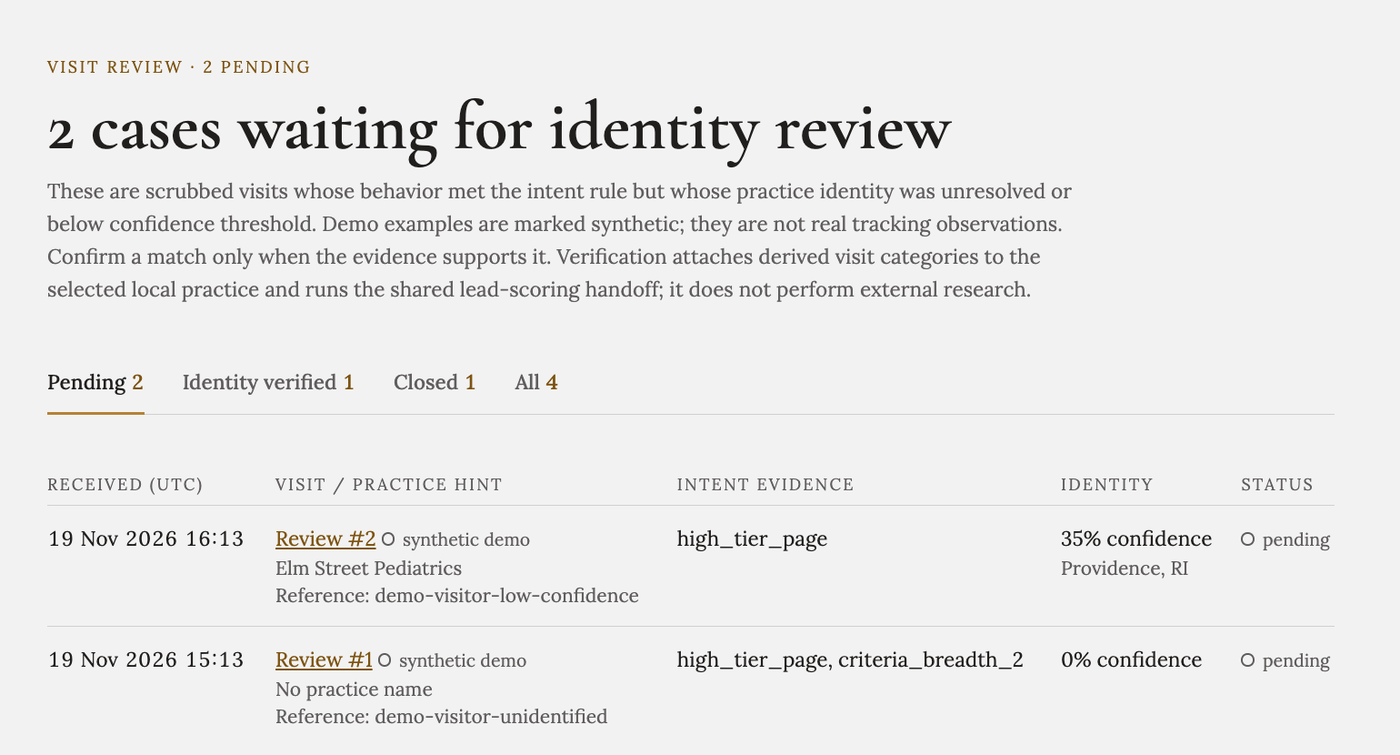
\includegraphics[width=0.72\textwidth]{demo-visit-review.png}
\caption{Demo, visit review queue: scrubbed visits that met the intent rule but whose practice is unknown or below the 0.5 confidence cutoff. Demo cases are labeled as synthetic.}
\label{fig:review}
\end{figure}

\subsection{Practice data and the research agent}

The National Provider Identifier registry lists who is licensed to provide care, but not what software a practice runs or where its website is, so the data work is split between a bulk table built ahead of time and an agent that works one lead at a time. The table holds 742 independent practices across 10 cities, pulled from the public registry with duplicate NPIs of one business merged, provider counts estimated, provenance recorded and stable NPI-based identifiers. The research agent is a Claude tool-use loop with two tools, a directory lookup over that table and a homepage check that fetches a candidate's HTTPS homepage and extracts only exact, recognized EHR names.

The agent's safeguards are code that the model cannot override, which is what makes an agent acceptable at this step. A candidate is matched automatically only with a score of at least 0.85 and a lead of at least 0.10 over the runner-up; an ambiguous case returns the top three candidates for a person to choose from; an EHR stays unknown unless the practice's own site names it; and the agent cannot introduce a practice that the directory did not return.

\subsection{Scoring}

The score is a logistic regression over 21 binary facts covering specialty, practice size, EHR, the pages visited and whether the last visit was in the past seven days. We chose it over a more flexible model deliberately: each fact multiplies the odds by a fixed amount and those amounts combine exactly into the prediction, so no score appears without its reasons. Since there are no real sales outcomes yet, a simulator generates 8,000 past leads, each won or lost by a rule the simulator keeps hidden, and each model version is fit on 5,600 of them and judged on the remaining 2,400. A hand-set points table built from the same facts (Appendix~\ref{app:points}) represents today's marketing baseline and is shown beside the model on every lead, so a rep can see where intuition and data disagree. Figure~\ref{fig:leads} shows the resulting ranked list and a single lead's page.

\begin{figure}[htbp]
\centering
\begin{subfigure}[t]{0.49\textwidth}
\centering
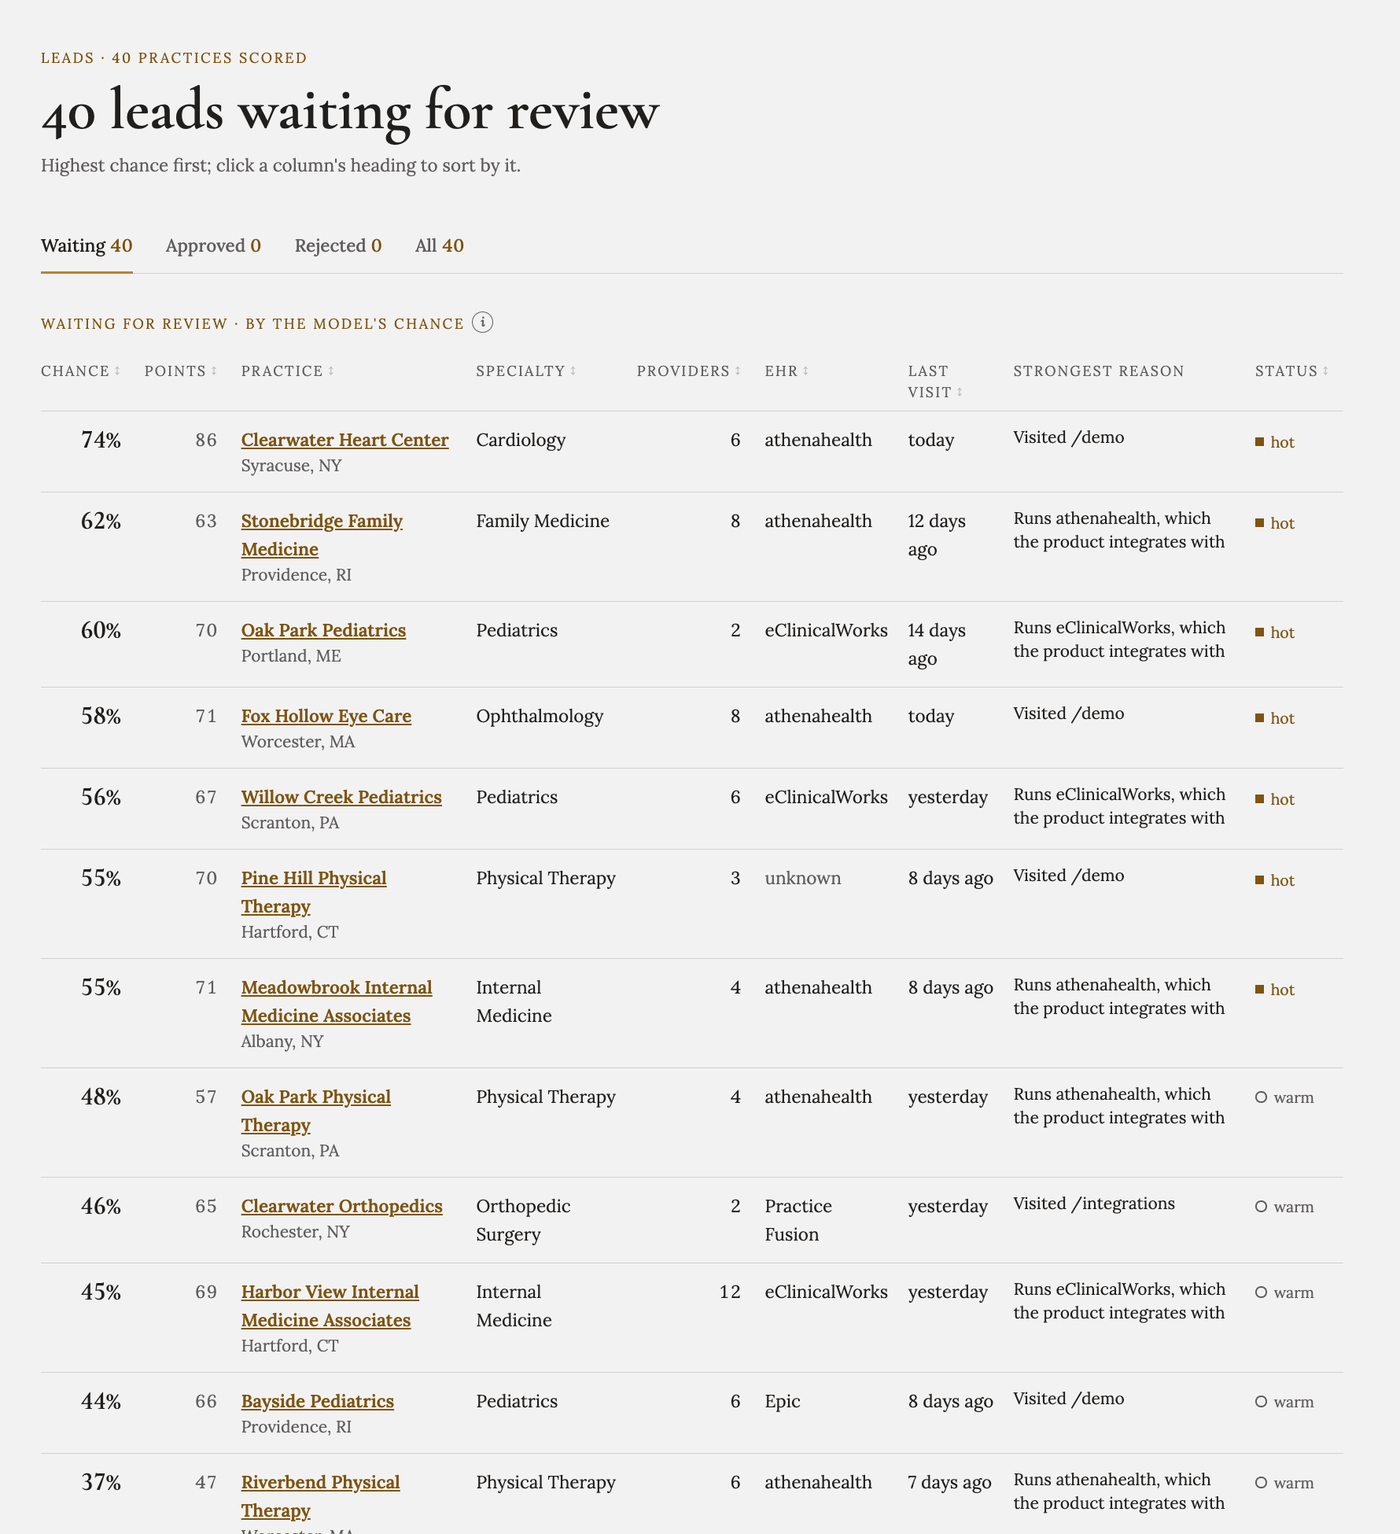
\includegraphics[width=\textwidth,trim=0 640 0 0,clip]{demo-leads.png}
\caption{Leads ranked by the model's chance, with the points score, practice facts and the strongest reason in each row.}
\end{subfigure}\hfill
\begin{subfigure}[t]{0.49\textwidth}
\centering
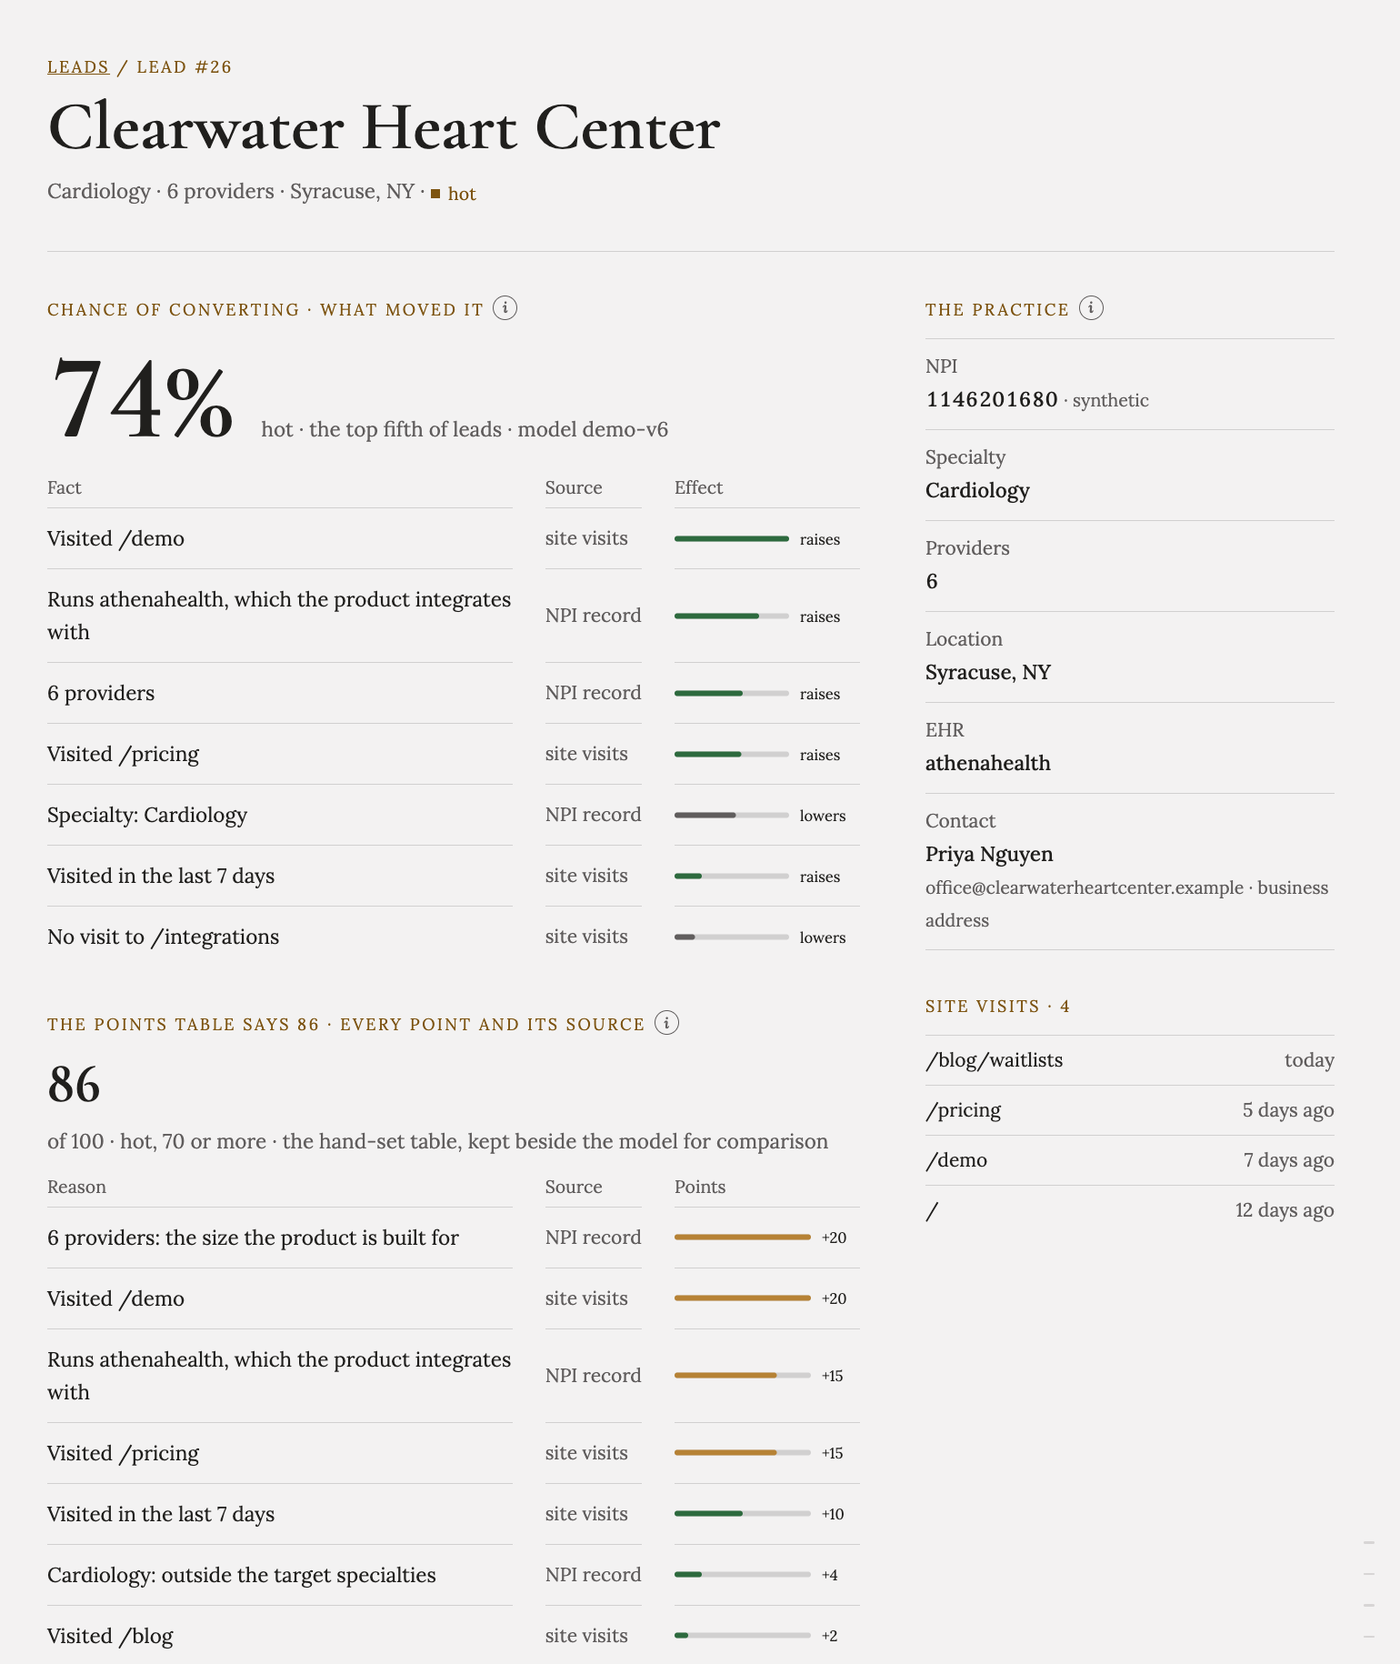
\includegraphics[width=\textwidth,trim=0 760 0 0,clip]{demo-lead-score.png}
\caption{One lead: a 74\% chance with every fact that moved it and its source, beside the practice record.}
\end{subfigure}
\caption{Demo, scoring as an SDR sees it.}
\label{fig:leads}
\end{figure}

New model versions are not trusted by default. A version is fit each simulated month and goes live only if it wins a four-measure scorecard against the live one, being worse than a small allowance on no measure and better on more measures than it is worse on; of six versions, one was sent back on a tie (Appendix~\ref{app:versions}).

\subsection{Writing, checks, approval and sending}

No email exists until an SDR asks for one, so a lead that is about to be rejected never gets one, while the call brief is available from the start. With an API key configured, Claude writes from the practice's name, specialty, provider count, city, state and EHR, the contact's name, the pages visited and the score's reasons; it is never given the contact's email address, the NPI or anything about patients. Code then checks the text before it is kept, rejecting patient information, claims the seller cannot support such as a guarantee or ``HIPAA certified,'' and any EHR or provider count that is not on the practice's record, and code rather than the model appends the CAN-SPAM footer. Without a key, the same button fills a template, which is what Figure~\ref{fig:decide}a shows.

\begin{figure}[htbp]
\centering
\begin{subfigure}[t]{0.49\textwidth}
\centering
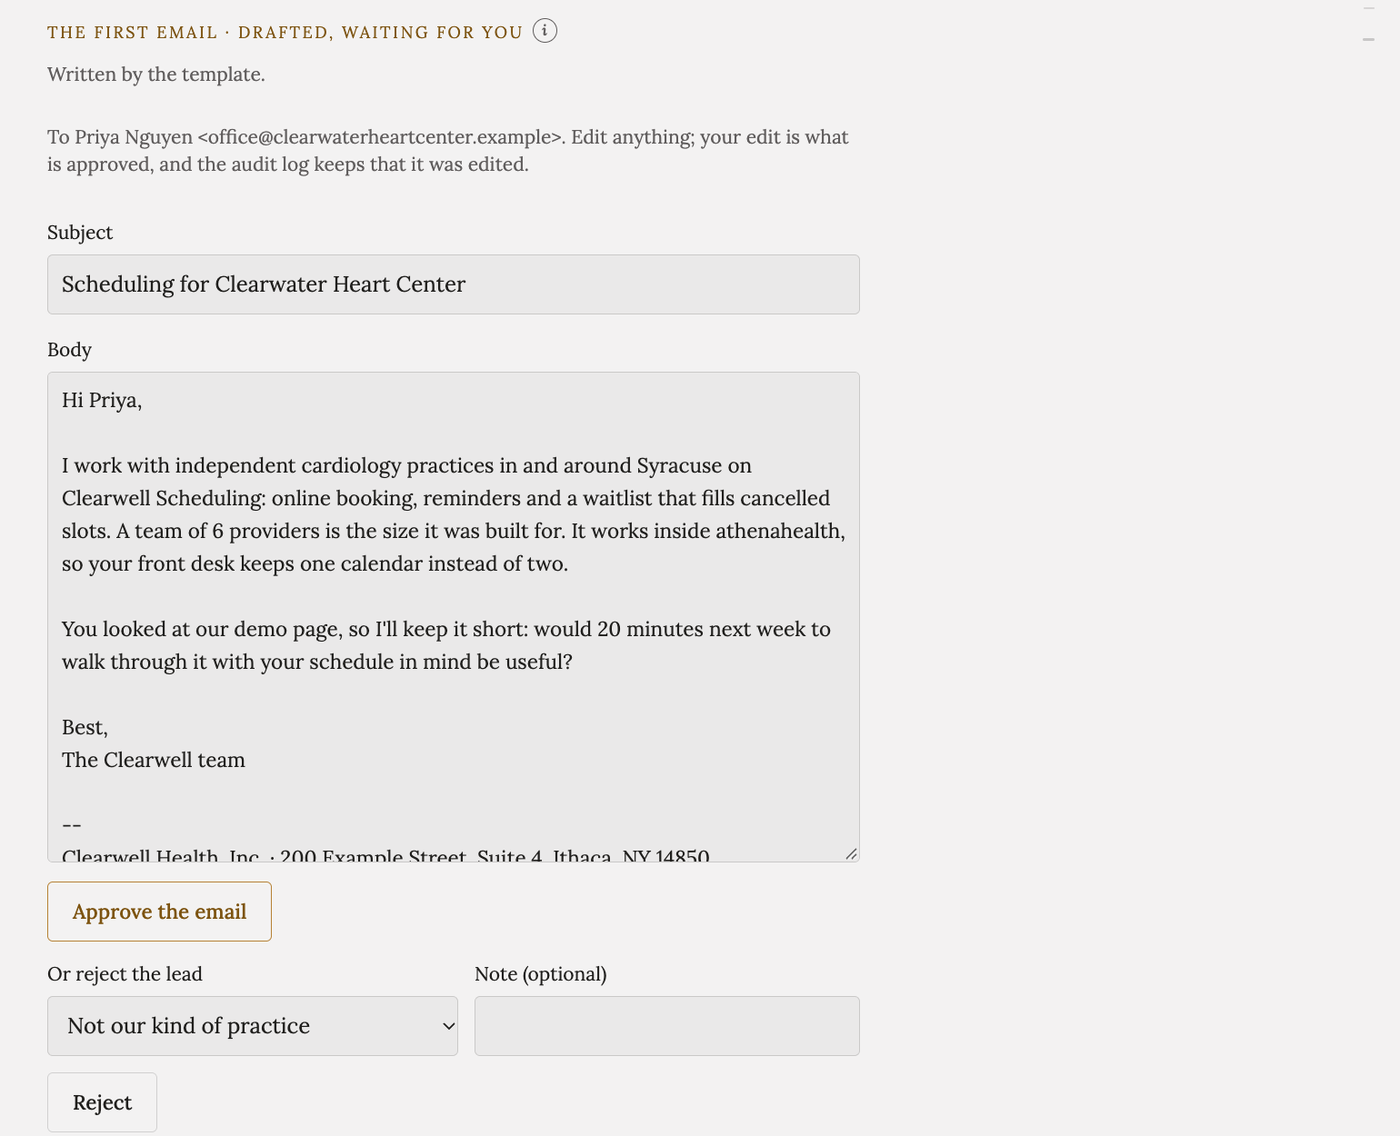
\includegraphics[width=\textwidth]{demo-lead-email.png}
\caption{The first email, drafted and waiting for the SDR; every word can be edited, and the edited text is what gets approved.}
\end{subfigure}\hfill
\begin{subfigure}[t]{0.49\textwidth}
\centering
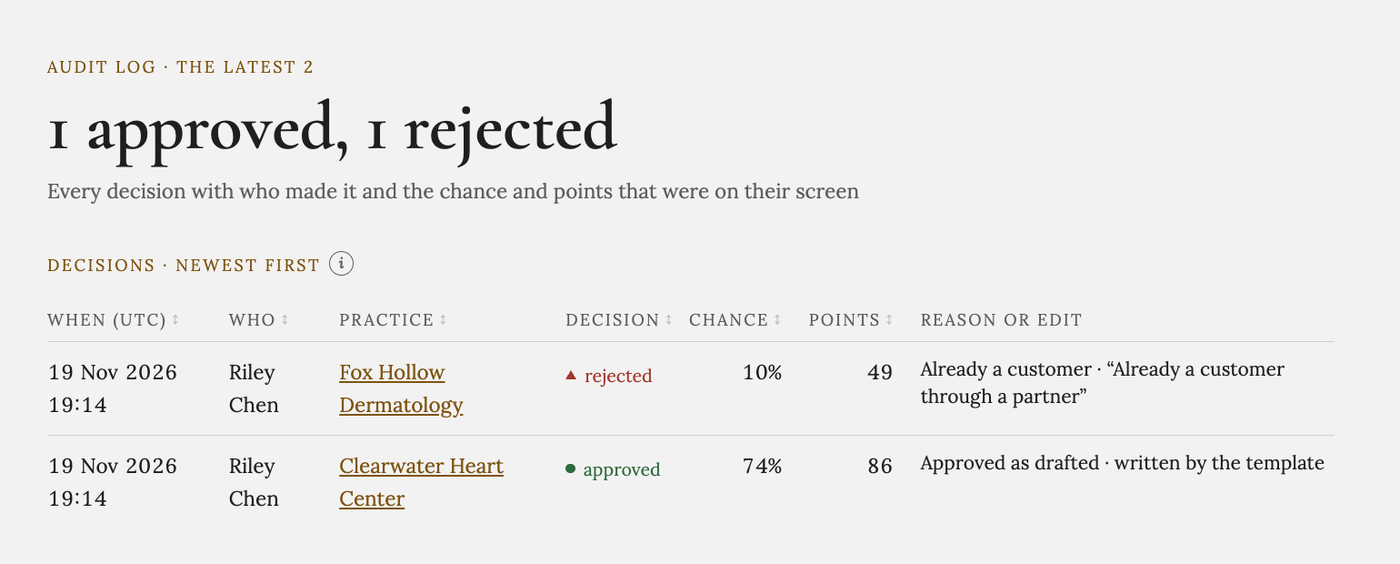
\includegraphics[width=\textwidth]{demo-audit-log.png}
\caption{The audit log as the sales manager sees it: who decided, when, the chance and points on screen, and the reason or edit.}
\end{subfigure}
\caption{Demo, the human decision and its record.}
\label{fig:decide}
\end{figure}

The SDR then approves the email, optionally after editing it, which reruns the checks, or rejects the lead with a reason and an optional note. If a colleague decided the same lead while it was open, the second decision is refused and the page shows the first. Every decision is written to an audit log that only the sales manager can read (Figure~\ref{fig:decide}b). Sending is the most recent addition: once a mailbox is configured, an approved email can be sent once, under the seller's header and logo, but only to a designated test address and never to the practice itself.

\section{AI tools}

AI appears in three places in the product, and the same principle governs each of them: use it where judgment or language is needed, and check its output with something that is not AI. The trained logistic regression, built with scikit-learn, is the system's predictive model; a gradient-boosted challenger is fit and reported on the same split but does not rank leads, since it is no more accurate and cannot explain a single prediction as simply. Claude, through the Anthropic Python SDK with \code{claude-opus-5-5} as the default model, writes the email and call brief and drives the research agent's tool loop. LangGraph runs the orchestration graph, though deliberately as a fixed state machine whose edges are chosen by code rather than as an agent framework. Each place where an LLM's output could cause harm has a code check behind it, namely the draft checks for the writer and the match safeguards for the agent, so a model error is caught before it reaches a practice or a score.

\section{Testing methodology}

We tested at three levels: automated tests of each module's behavior, a simulated ground truth for the gate and practice matching, and a held-out benchmark for the scorer. The repository's 177 automated tests, all passing at the time of writing, cover the gate and its privacy boundary, the review queue, the research agent's safeguards against a fake directory, each of the graph's seven outcomes, the NPI adapter, the draft checks, roles and sending, and they never call the Anthropic API or open a mail connection, so they are deterministic and free to run.

The gate and the matching cannot be judged without knowing the right answer for each visitor, so the evaluation uses a persona simulator whose ground truth is generated separately and never enters lead state. It creates 2,000 visitors from five personas (browsers 45\%, researchers 20\%, ready-to-buy visitors 10\%, administrators 15\% and owners 10\%) over 400 synthetic practices, labels browsers as should-not-pass and everyone else as should-pass, and samples whether each visitor is identified from assumed rates for each persona. From this we measure gate recall, browser false passes, page-category accuracy and match accuracy. Matching was then rerun on real registry names: each of the 742 practices is queried with four name forms (the registry name, the name without its legal suffix, a casual form and a typo), each with and without a location, which gives 4,152 queries for practices in the directory and 1,784 for the 30\% of practices held out of it.

The scorer is judged on the 2,400 simulated leads it never trained on, against a random pick, the points table and the challenger, using four measures: conversion in the top tenth, which is what a team calls first; AUC, which judges the whole ranking; average precision, which measures how tightly converters cluster at the top; and calibration error, which checks whether a 30\% chance means about 30 conversions in 100. The most important caveat of this methodology is that the simulator's hidden rule is ours, so the benchmark tells us whether the scorers recover a known pattern and how they compare with one another, not how any of them would perform on real sales.

\section{Results}
\label{sec:results}

\subsection{Scoring}

As Figure~\ref{fig:odds} shows, the model learned a sensible structure from the simulated history. Visiting the demo page, having 2 to 10 providers and running an EHR the product integrates with each roughly triple the odds of converting, while running Epic or having 26 or more providers each cut them by more than half. The model also corrected two of the hand-set table's guesses: the table ranks Dermatology third among the named specialties and treats Epic like any other EHR, whereas the model places Dermatology below Internal Medicine ($\times$0.78 against $\times$1.10) and finds that Epic more than halves the odds ($\times$0.42).

\begin{figure}[htbp]
\centering
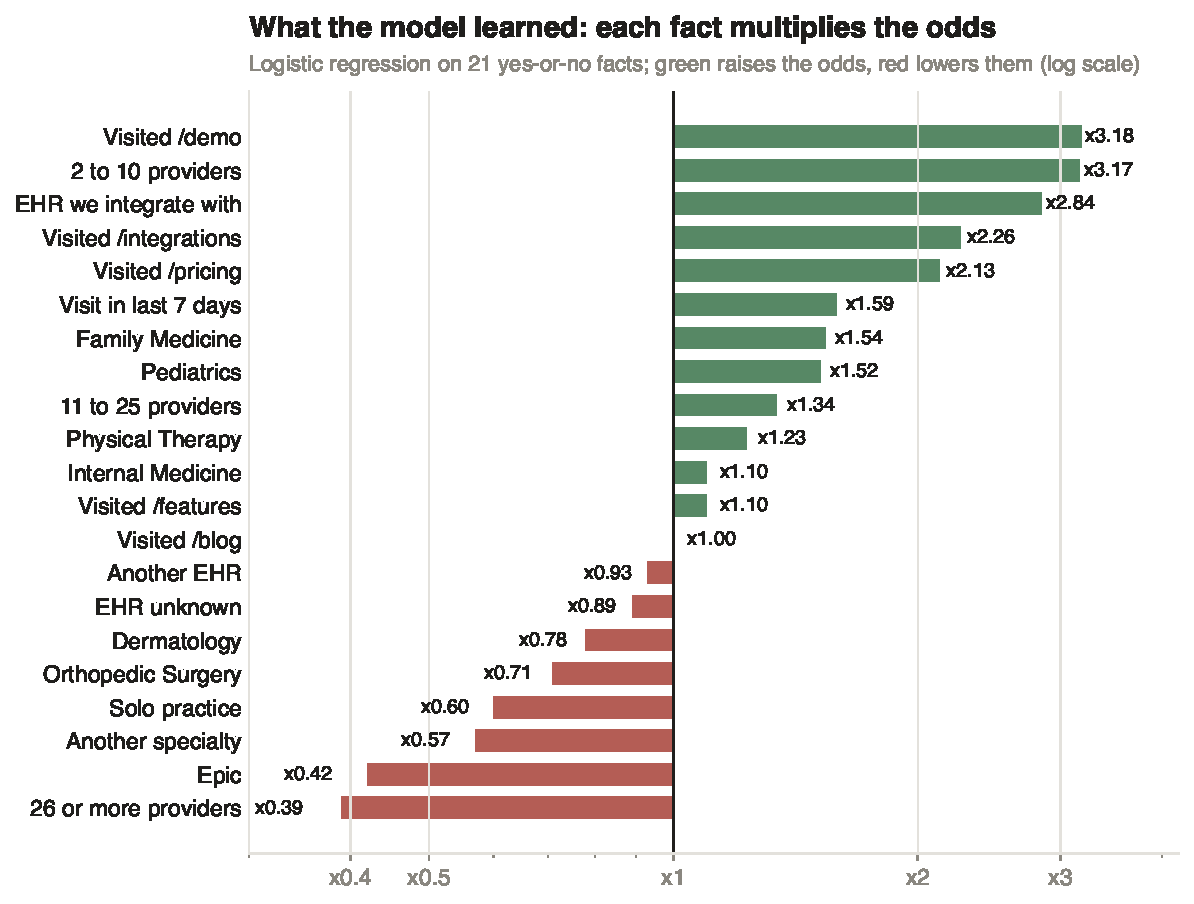
\includegraphics[width=0.6\textwidth]{chart-odds.pdf}
\caption{Odds multiplier for each of the 21 facts in the live model.}
\label{fig:odds}
\end{figure}

According to Table~\ref{tab:bench}, the model's top tenth converts at 77.9\% (187 of 240 leads) against a 28.7\% base rate, a 2.72$\times$ lift, while the points table reaches 75.4\% (181 of 240) and the challenger 78.3\%. The model's edge over the points table is real but small, 78 against 75 in 100, which is why the table remains on the page beside it rather than being retired. Calibration matters as much as ranking here, since an SDR reads the chance as a number. Splitting the held-out leads into six equal groups by predicted chance (Figure~\ref{fig:bench}), the stated chance stays close to what actually converted: when the model said 45\%, 42\% converted, and when it said 68\%, 72\% did. Across the six versions, more history mostly made the chances more honest rather than the ranking sharper, as top-tenth conversion stayed between 75\% and 79\% while calibration error fell from 2.5 to 1.7 points.

\begin{table}[htbp]
\centering
\small
\caption{Benchmark on 2,400 held-out simulated leads (28.7\% convert overall).}
\label{tab:bench}
\begin{tabular}{@{}lccc@{}}
\toprule
 & Points table & Trained model & Challenger \\
\midrule
Conversion in the top tenth & 75.4\% & 77.9\% & 78.3\% \\
Lift over a random pick & 2.63$\times$ & 2.72$\times$ & 2.73$\times$ \\
AUC & 0.793 & 0.810 & 0.805 \\
Average precision & 0.616 & 0.656 & 0.644 \\
Calibration error & n/a & 1.7 points & 1.9 points \\
Role in the app & Shown beside the model & Ranks the leads & Reported, not used \\
\bottomrule
\end{tabular}
\end{table}

\begin{figure}[htbp]
\centering
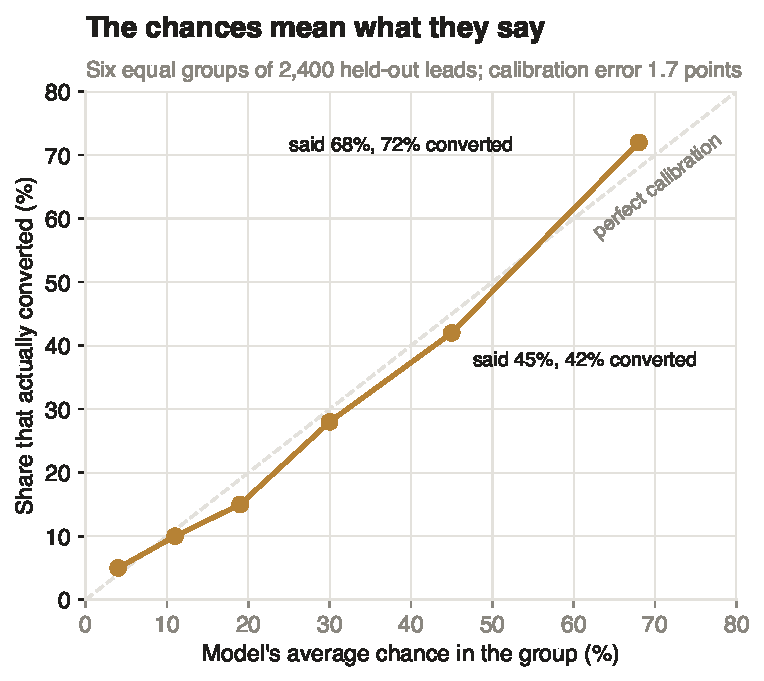
\includegraphics[width=0.5\textwidth]{chart-calibration.pdf}
\caption{Calibration on the 2,400 held-out simulated leads, in six equal groups by predicted chance.}
\label{fig:bench}
\end{figure}

\subsection{What testing changed}

Testing did not merely confirm the design; it changed it three times, as Figure~\ref{fig:iter} shows. The first page taxonomy let 15.7\% of identified browsers through the gate, because a blog post about pricing looked like a pricing page and a careers posting for a billing specialist looked like a billing page. Classifying pages by site section before keywords reduced browser false passes to 0\% and raised should-pass recall from 95.0\% to 95.4\%, although the perfect page-category accuracy behind that result was measured on the same simulated catalog the fix was written for, so what carries over to real traffic is the rule rather than the number. Second, real registry names carry legal suffixes, initials and conjunctions, so obvious matches failed; normalizing them raised correct matches from 63.1\% to 91.5\% on real NPI names with no wrong matches. Third, the simulation showed that unresolved identity rather than the gate's rules is the main bottleneck, since 103 of 309 future converters (33.3\%) failed the gate first on identity, which is what led to the review queue that now keeps 300 of the 2,000 simulated visitors who would otherwise have been dropped.

\begin{figure}[htbp]
\centering
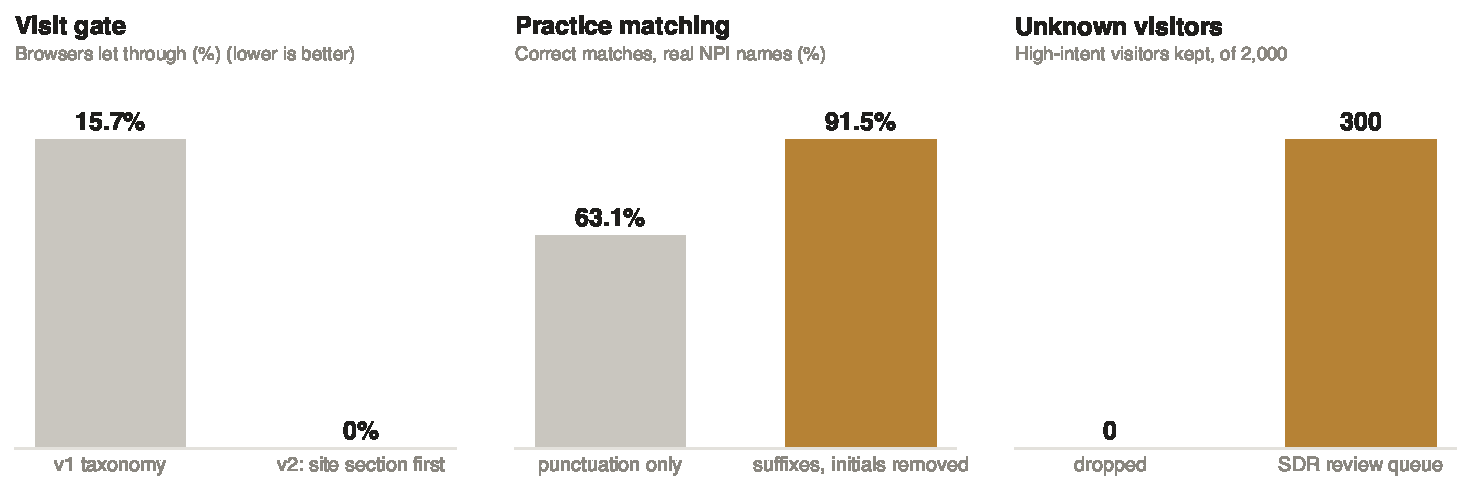
\includegraphics[width=0.88\textwidth]{chart-iteration.pdf}
\caption{Three design changes driven by testing. The gate and review results use 2,000 simulated visitors; the matching result uses queries generated from real NPI registry names.}
\label{fig:iter}
\end{figure}

The matching cutoff is itself a trade-off, and Figure~\ref{fig:match} shows where the current one sits. Lowering the automatic-match threshold to 0.75 would match 96.0\% of practices that are in the directory, but it would also attach 6.1\% of queries for absent practices to the wrong business, whereas a threshold of 0.90 cuts that to 1.5\% at the cost of matching only 82.3\%. We kept 0.85 with a 0.10 margin, which matches 91.5\% correctly and falsely matches 2.4\% of absent-practice queries, since a wrong match sends an SDR to the wrong practice with the wrong facts, which is worse than handing an ambiguous case to a person.

\begin{figure}[htbp]
\centering
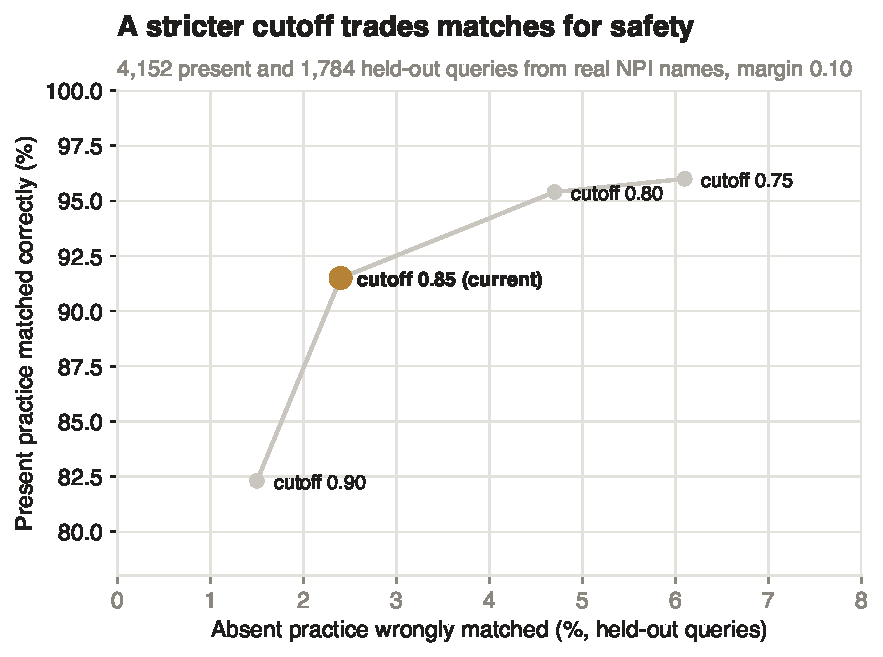
\includegraphics[width=0.5\textwidth]{chart-matching.pdf}
\caption{Correct matches against false matches on held-out practices, by automatic-match cutoff.}
\label{fig:match}
\end{figure}

\subsection{Estimated business impact}

Assuming the measured case's time per lead and conversion rate hold, most of the value comes from reach: with the automated steps an SDR spends about 14.6 minutes per lead instead of 30, so the same 12 SDRs can work about 1,031 leads a month instead of 500. Applying only the model's small edge over the points table (1.03$\times$) gives about 77 new practices a month instead of 36, and applying the full 2.72$\times$ lift gives about 202, or roughly \$5.9 million to \$23.9 million in added contract value a year at \$12,000 per practice. Since the high estimate assumes today's leads are no better than random, which is unlikely, the low estimate is the more defensible figure.

\section{Ethical considerations}

The first ethical constraint is privacy, and the design keeps patient data out by construction rather than by policy. Only public business facts reach a model, namely the NPI registry, a practice's own homepage and company-level visit behavior; the writer is never given an NPI, an email address or anything about patients, and code rejects any draft that mentions patient information. This is also what keeps outreach a CAN-SPAM matter rather than a HIPAA one, which is why every email carries a postal address and an opt-out. The remaining gap is at ingestion: the visit endpoint relies on the caller's assertion that the data has been scrubbed and stops any visit not marked that way before research can run, but no scrubber exists yet, so the system must not receive real visit data until one does.

The second is accountability. No AI sends anything; a named SDR approves every email, the sales manager can audit every decision together with the chance and points that were on screen, and two people cannot decide the same lead at once. Code also guards against the failure LLMs are best known for, inventing facts, by rejecting any EHR or provider count that is not on the record. Explainability supports the same goal, since a rep who can see that a score rests on a demo-page visit and a matching EHR is in a position to disagree with it, and the points table beside the model makes such disagreement visible.

The third concerns fairness in who gets contacted. A model that learns which practices convert will, by design, deprioritize the practices that converted less, and in our model that includes solo practices ($\times$0.60) and some specialties. With real data, such patterns could reflect where the product happened to be sold before rather than where it would help, and could steer a seller away from small or rural practices that have the fewest alternatives. Since our labels currently come from a rule we wrote, the model encodes our own assumptions; once real outcomes exist, the score's error rates should be checked by practice size, specialty and region before it is relied on.

Finally, visitor identification should stay at the company level, with the tracking source and data retention agreed before any real data flows, and the time savings estimated above could be framed either as more conversations for the same team or as roughly 13 avoided hires; that choice belongs to the seller rather than the tool.

\section{Limitations and planned work}

The largest limitation is that every outcome is simulated. The scorer learns a rule we wrote, the visits come from personas we defined with assumed identification rates, and the gate's zero false-pass rate was measured on the same URL catalog its fix was written for, so none of these numbers are evidence of real-world performance. The second limitation is integration. The research agent and the LangGraph graph work together and have tests for every outcome, but the web app does not call them yet, so the demo matches practices by exact local name instead of researching them. The NPI table also contains no EHR or website data, so the homepage check needs a separately supplied and validated domain, and 2.4\% of queries for practices missing from the table still match the wrong business.

Several further pieces are designed but not built, and each follows the architecture notes: connecting the orchestration graph to the web app with per-step traces and retries, an ingestion-time patient-data scrubber and an approved identity source, a single Claude call that summarizes a visitor's intent, retraining on SDR approvals and rejections through the same scorecard, and Claude's own ranking of the held-out leads as a benchmark row, which would finally answer the proposal's question of whether transparent ML outranks an LLM's judgment. The deployed demo also rebuilds its database on a cold start, so decisions can reset between visits.

\section{Conclusions}

LeadFinder shows that most of a sales-prospecting pipeline does not need an LLM, and that the parts that do are safer when they are bounded and checked by code. The gate, the matching safeguards, the draft checks and the orchestration are plain rules; a transparent logistic regression ranks the leads with a 2.72$\times$ lift and honest chances on simulated data; Claude is used where language and judgment matter, writing on request and researching under a ten-call cap; and a person decides every email. Testing changed the design three times, each time in a way that reasoning alone would not have found. Assuming the next goal is evidence that the system works on real sales, the work that matters most is not a better model but real inputs: a scrubbed visit feed, the research path wired into the app, and SDR decisions flowing back as labels, so that the comparison with an LLM's judgment can finally be run on outcomes that are not our own.

\section*{AI attribution}\label{sec:ai-attribution}

This report was written by Claude (Anthropic's Claude Opus 5.5, through Claude Code), including its prose, tables, diagrams and charts, and the demo screenshots were captured by Claude from a local run of the application. It is based on the team's own inputs and information: the project's code and commit history, the evaluation and matching reports, the proposal and brainstorm documents, the course rubric, and the team's presentation deck. Some of that source material was itself produced with Claude earlier in the project, most notably the final presentation deck and parts of the project documentation, so in those places the report restates content that originated with the AI rather than independently with the team. Figures and results were checked against the running application, the test suite and the generated evaluation reports, and the team remains responsible for the accuracy of the final submission.

\appendix
\section{The hand-set points table}
\label{app:points}

\begin{table}[H]
\centering
\small
\caption{The points table kept beside the model, built from the same 21 facts.}
\begin{tabularx}{\textwidth}{@{}p{2.2cm}L@{}}
\toprule
Fact & Points \\
\midrule
Specialty & Family Medicine 20, Pediatrics 18, Dermatology 16, Internal Medicine 15, Orthopedic Surgery 12, Physical Therapy 10, other 4 \\
Providers & 2 to 10: 20; 11 to 25: 10; solo: 4; 26 or more: 0 \\
EHR & One the product integrates with 15, unknown 5, any other 0 \\
Pages visited & Demo 20, pricing 15, integrations 8, features 4, blog 2; capped at 40 \\
Recency & A visit in the last 7 days: 10 \\
Bands & Total 0 to 100; hot at 70 or more, warm at 45 or more, otherwise cool \\
\bottomrule
\end{tabularx}
\end{table}

\section{Model versions and the scorecard}
\label{app:versions}

\begin{table}[H]
\centering
\small
\caption{Six monthly model versions, each judged on the same 2,400 held-out leads.}
\begin{tabular}{@{}lrccccl@{}}
\toprule
Version & Fitted on & Top tenth & AUC & Avg.\ precision & Calibration & Outcome \\
\midrule
demo-v1 & 600 & 75.4\% & 0.802 & 0.641 & 2.5 pts & Was live \\
demo-v2 & 1,600 & 79.2\% & 0.809 & 0.653 & 2.6 pts & Was live \\
demo-v3 & 2,600 & 77.9\% & 0.811 & 0.653 & 2.0 pts & Was live \\
demo-v4 & 3,600 & 76.7\% & 0.811 & 0.653 & 1.7 pts & Sent back on a tie \\
demo-v5 & 4,600 & 77.5\% & 0.811 & 0.655 & 1.7 pts & Was live \\
demo-v6 & 5,600 & 77.9\% & 0.810 & 0.656 & 1.7 pts & Live \\
\bottomrule
\end{tabular}
\end{table}

\begin{figure}[H]
\centering
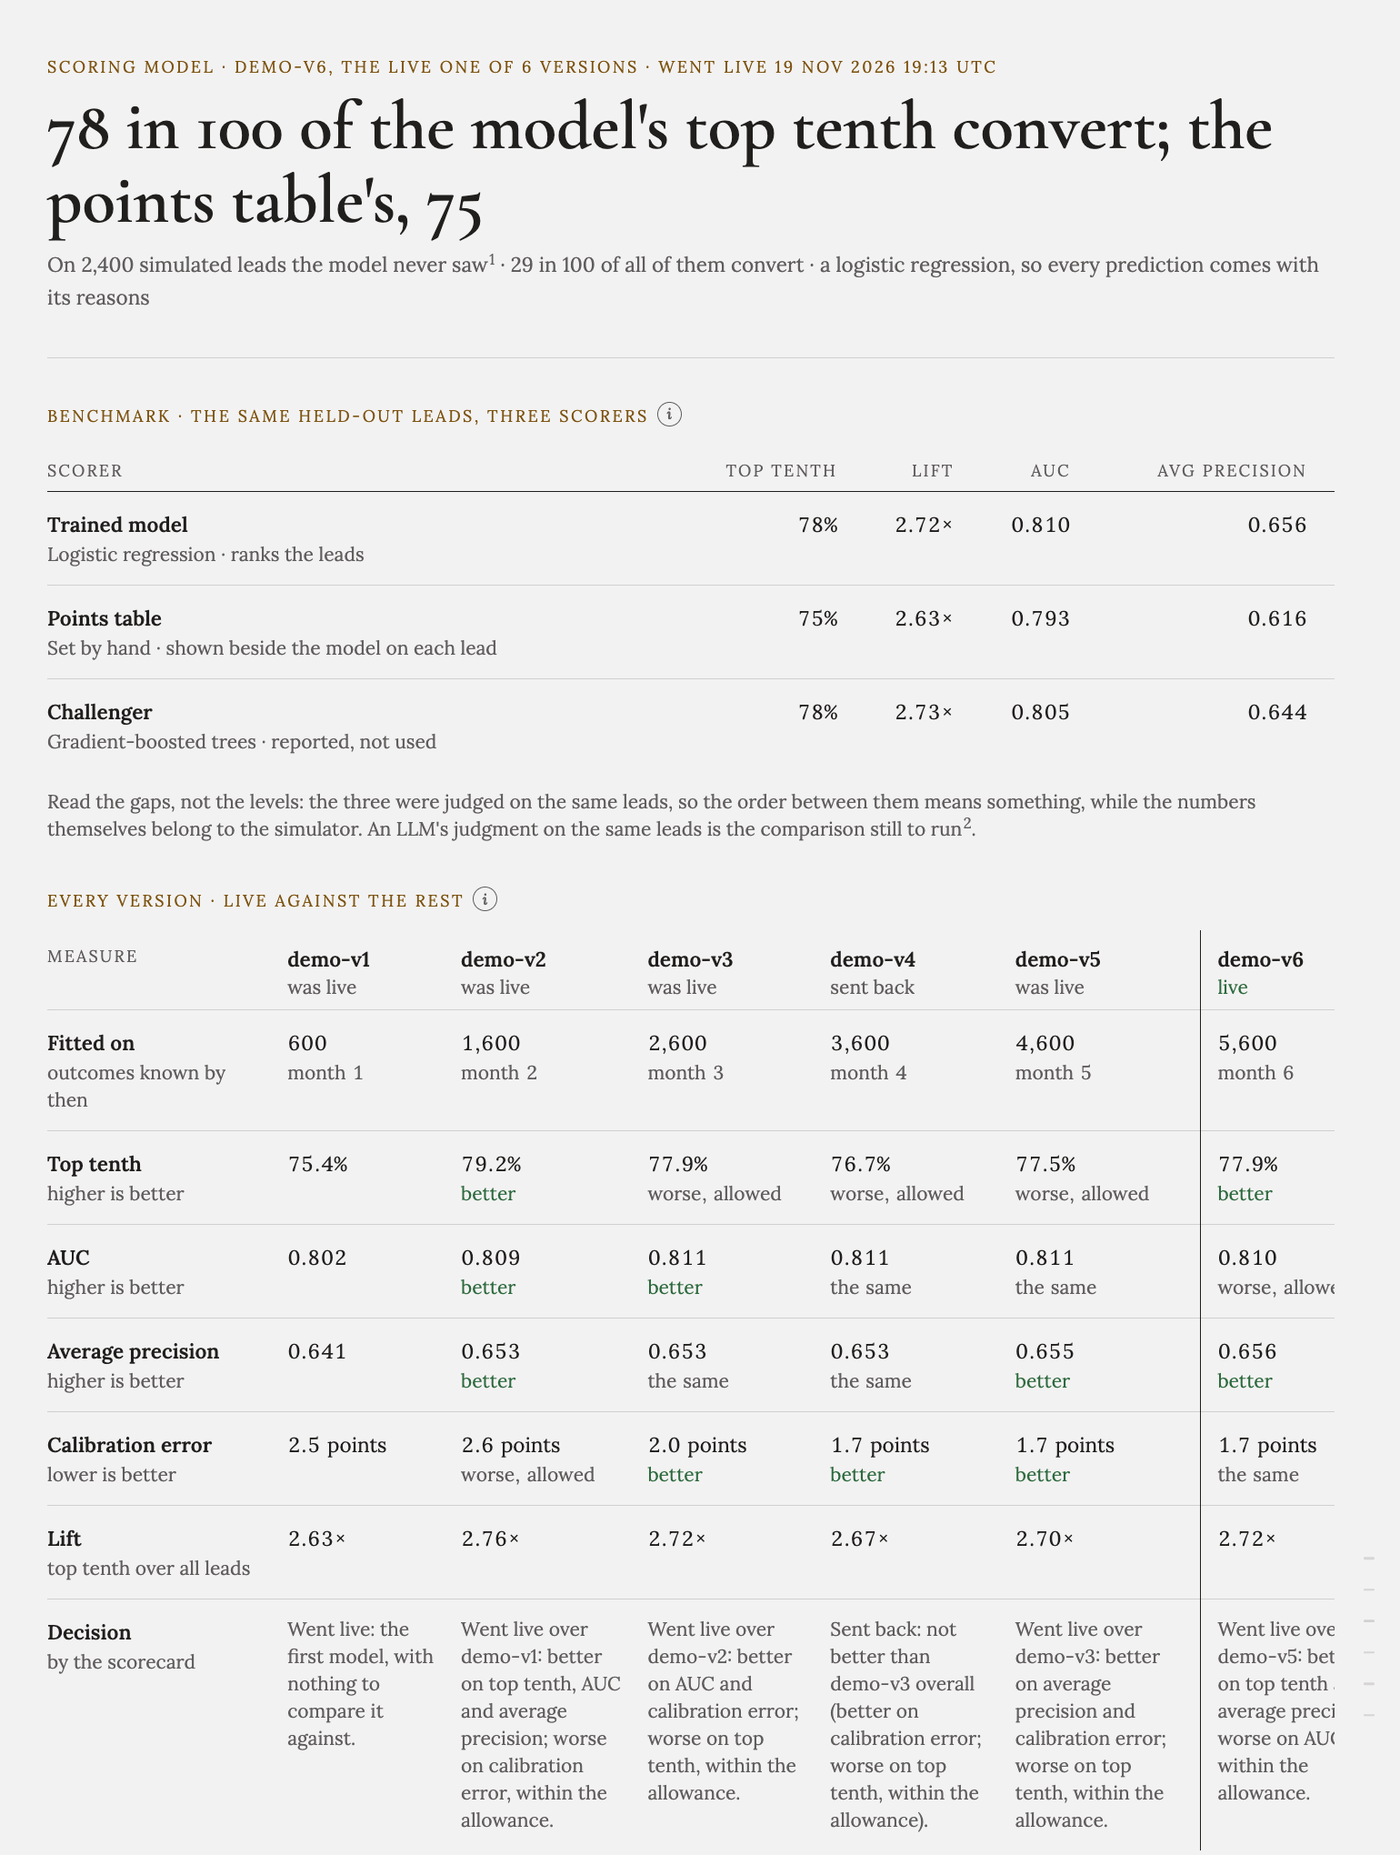
\includegraphics[width=0.7\textwidth]{demo-scoring-model.png}
\caption{Demo, scoring model page: the benchmark, every version against the live one, and the scorecard's decision on each.}
\end{figure}

\section{Reproducing the results}

{\sloppy The demo screenshots were taken from a fresh local database with the template writer, following the run instructions in the repository's README. The test suite runs with \code{python -m pytest -q}. The gate, taxonomy and matching evaluation is produced by \code{python -m leadfinder.evaluation --n 2000 --seed 42}, which writes \code{docs/evaluation-report.md}, and matching on real NPI names by \code{python -m leadfinder.evaluation.npi\_match --seed 42}, which writes \code{docs/npi-match-report.md}. The charts are drawn by \code{docs/report-assets/make\_charts.py}, and the architecture and workflow diagrams are hand-written SVG files in the same folder. This report is typeset from \code{docs/technical-report/technical-report.tex} with \code{tectonic}.\par}

\end{document}
